\pagestyle{fancy}

\graphicspath{ {Figures/Chapter1_Overview/} }

\section{CERN accelerators complex}
\label{sec:CERN_acc_complex}

The European Organization for Nuclear Research (CERN) was founded in 1954, and it has become the largest particle physics laboratory in the world \parencite*[][]{ref:CernWebsite}. It sits astride the FrancoSwiss border near Geneva. It was one of Europe's first joint ventures and now has 23 member states. At CERN, the world's largest and most complex scientific instruments are used to study the basic constituents of matter, but the physics program at the laboratory is much broader, ranging from nuclear to high-energy physics, from studies of antimatter to the possible effects of cosmic rays on clouds.

CERN has not only provided advancements in fundamental sciences but has also pushed the frontiers of technology, with inventions such as the world wide web (www), Positron Emission Tomography (PET), etc. which have a positive impact on society globally.

CERN's accelerator complex (See \ref{fig:AccComplex} ) consists of many different types of linear and circular accelerators and interconnecting transfer lines to gradually accelerate the particles before injection into the Large Hadron Collider (LHC). 

Since 2020, Linear accelerator 4 (Linac4) became the source of proton beams for the LHC. Linac4 is an 86 \si{\meter} long machine. It accelerates negative hydrogen ions up to 160 \si{\mega \electronvolt}. The ions are then stripped of their two electrons during injection from Linac4 into the Proton Synchrotron Booster (PS Booster or PSB) to leave only protons. The PS Booster is made up of four superimposed synchrotron rings, with a 157 \si{\meter} circumference, which accelerates the injected protons up to 2 GeV for injection into the Proton Synchrotron (PS). 

Currently, the PS is the oldest accelerator in the chain. With a circumference of 628 meters, the PS operates up to 26 \si{\giga \electronvolt}. The Super Proton Synchrotron (SPS) is the second largest machine in the complex, measuring nearly 7 \si{\kilo \meter} in circumference. It takes the particles from the Proton Synchrotron and accelerates them up to 450 \si{\giga \electronvolt}. The CERN accelerator complex culminates with the Large Hadron Collider. The LHC consists of a 27 \si{\kilo \meter} ring of superconducting magnets, which guide two high-energy particle beams traveling in the opposite directions in separate beam pipes. The beams collide at four locations around the accelerator ring, corresponding to the positions of four particle detectors ATLAS, CMS, ALICE and LHCb. The High Luminosity Large Hadron Collider ( HiLumi LHC) project aims to deliver proton-proton collisions at 14 \si{\tera \electronvolt}.

\begin{figure}[h]
    \centering
    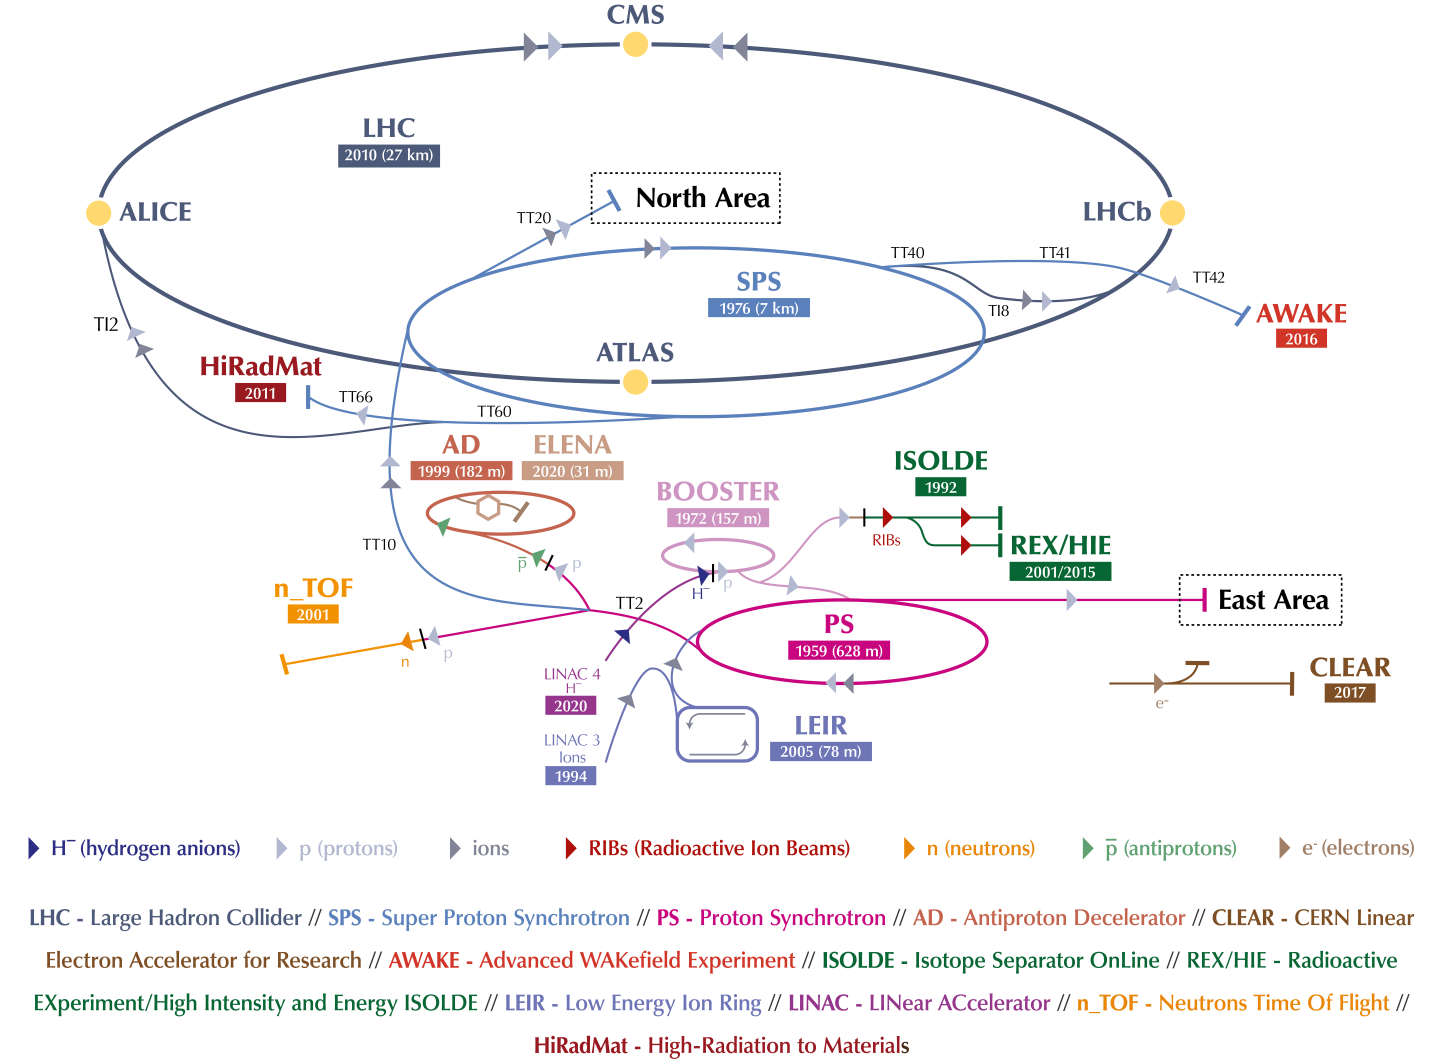
\includegraphics[width=0.95\columnwidth]{Figure_AcceleratorChain/cernComplex.png}
    \caption{CERN Accelerator Complex \parencite*[][]{ref:cerncomplex} . }
    \label{fig:AccComplex}
\end{figure}

Not only protons can be accelerated at the CERN accelerator complex. Linear accelerator 3 (Linac 3) is the starting point for the ions. It provides mainly lead ions, but also argon and xenon were used in the past. Experiments with oxygen are planned for the future. The long pulses of lead ions from Linac 3 are transformed into short, dense bunches by the Low Energy Ion Ring (LEIR) before they are injected into the PS. 

The injector chain apart from feeding the LHC is also used to deliver particles to several other experiments carried out at CERN, including Antimatter research on the Antiproton Decelerator (AD) and Extra Low ENergy Antiproton (ELENA), radioactive ion beam research on ISOLDE, research on neutron-nucleus interactions on the n-TOF facility, research on radiation-induced damage on materials in the HiRadMat facility and even studies on the use of proton-driven plasma wake-fields in AWAKE. 

\section{Linear Accelerator 4 (LINAC4)}
\label{sec:LINAC4}

As part of the LHC injection upgrade (LIU), CERN approved in 2007 the construction of LINAC4, to substitute the, by then existent, LINAC2 accelerator. The main goal for the construction of LINAC4 was to increase the beam brightness out of the PSB by a factor of 2, making possible an upgrade for the LHC injectors for higher intensity and eventually an increase of LHC luminosity \parencite*[]{ref:LIU}. 

The increase in beam brightness is achieved by combining two effects, the increase of the top energy to \SIlist[]{60}{\mega \electronvolt} (compared to the \SI[]{50}{\mega \electronvolt} given by LINAC2), which reduces significantly the space charge effect causing emittance blow up in the PSB. Secondly, the use of $H^{-}$ ions instead of protons makes it possible to inject into the PSB via the charge exchange scheme, which is explained in detail in Chapter \ref{ch:H0Hm}.

\begin{figure}[h]
    \centering
    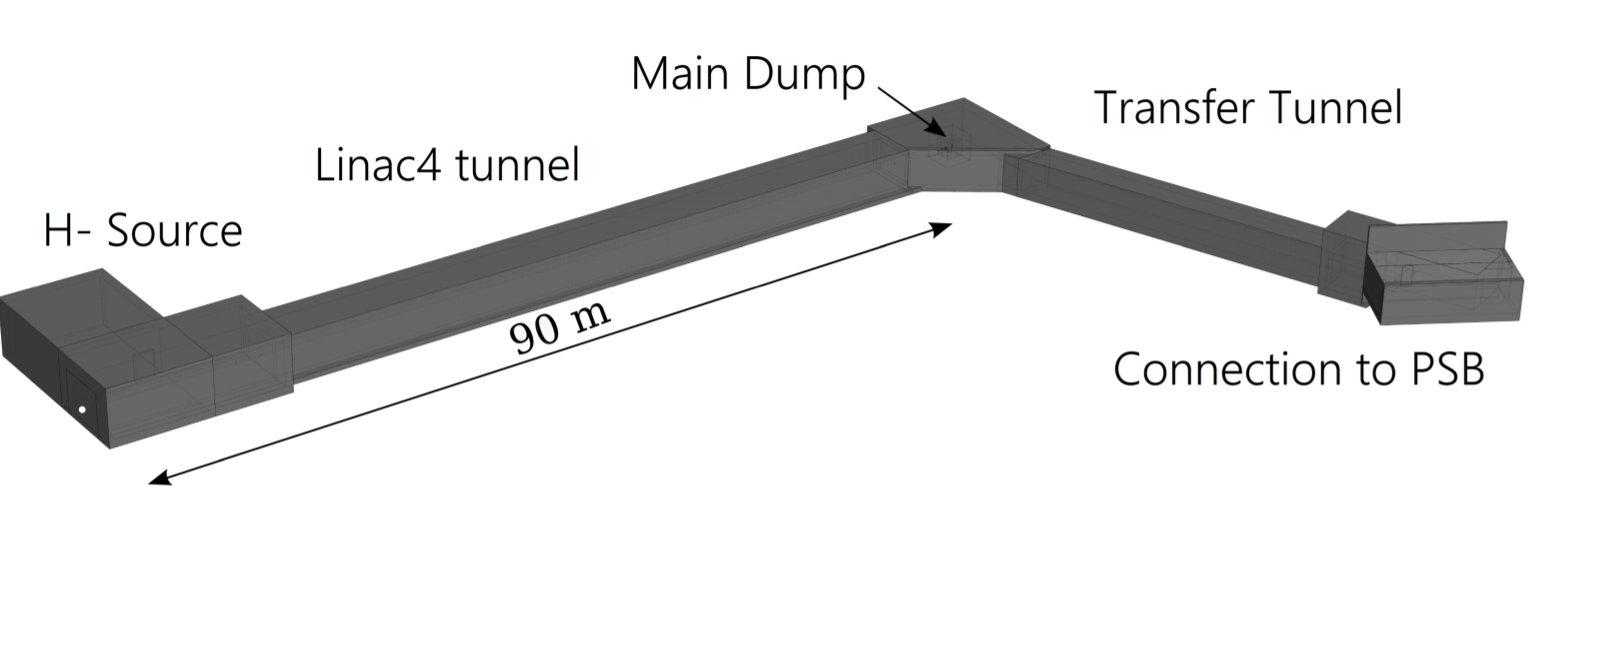
\includegraphics[width=0.70\columnwidth]{Linac4_Layout/linac4_Layout.png}
    \caption{General Layout of LINAC4 and its transfer-line to the PSB. }
    \label{fig:Linac4_layout}
\end{figure}

LINAC4 is \SI[]{86}{\metre} long and is located 12 m below ground. Figure \ref{fig:Linac4_layout} shows the source, tunnel, dump and transfer line to the PSB. Beams began to be produced in 2013 and the milestone energy of \SIlist[]{160}{\mega \electronvolt} was reached in 2016, after the commissioning of all the accelerating structures. During the long shut-down (2019-2020), LINAC4 finally replaced LINAC2 as the source of protons for the LHC. 

A more detailed description of the architecture of the accelerating section of LINAC4 is shown in figure \ref{fig:Linac4_acc}. The accelerating sequence is quite standard for a pulsed LINAC design. The LINAC4 source is a cesiated molybdenum-surface radio-frequency plasma ion source \parencite*[][]{ref:SourceCite}. This source can produce $H^{-}$ ion beams of up to 400\si[]{\micro \second} pulse length, 40\si[]{\milli \ampere} at a maximum revolution frequency of \SI[]{0.8}{\hertz}

\begin{figure}[h]
    \centering
    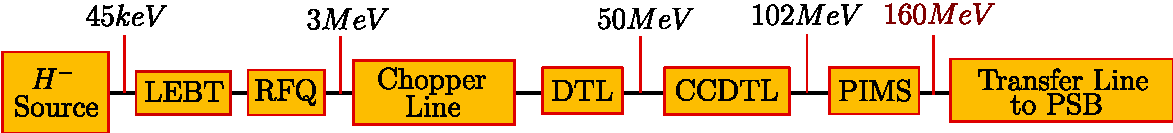
\includegraphics[width=1.0\columnwidth]{Linac4_AcceleratingPart/Linac4_acc.pdf}
    \caption{LINAC4 accelerating components layout. }
    \label{fig:Linac4_acc}
\end{figure}

The Low Energy Beam Transport (LEBT) line provides the beam matching from the source to the RFQ (Radio Frequency Quadrupoles) and contains the diagnostics to monitor the source. The three meter RFQ performs the beam capture and bunching and accelerates the particles to an energy of 3\si[]{\mega \electronvolt}. It is followed by a Medium Energy Beam Transport (MEBT) or "Chopper Line". This system consists of an electrostatic beam deflector followed by a beam dump. The purpose of this line is to avoid losses at higher energies when the induced radiation is higher. 

Three types of losses are treated with this system. Firstly, losses due to instable LINAC4 pulses. Secondly, it can be used to clean the first few tens of \si[]{\micro \second} of the beam pulse which are generally not stable. Finally, its purpose is to create "holes" in the beam pulse, timed with the rise-time of the PSB distributor, which switches the incoming LINAC4 beam between the four Booster Rings.  

The chopping line is followed by a series of three accelerating structures. The Drift Tube Linac (DTL) is divided in three tanks and accelerates the beam up to 50\si[]{\mega \electronvolt}. The Cell-Coupled Drift Tube Linac (CCDTL) is made of 7 accelerating modules for a top energy of 102 \si[]{\mega \electronvolt}. Finally, the Pi-Mode Structure (PIMS) brings the energy of the beam to the desired 160 \si[]{\mega\electronvolt}. More information about LINAC4 and its conforming parts can be found in \parencite*[]{ref:Linac4Technical}.  

In the current operational conditions, the LINAC4 pulse structure consists of four individual macro pulses, typically 20 - 100  \si[]{\micro \second}long (depending on the required number of injected turns per ring) and separated by a 1 \si[]{\micro \second} particle-free gap (See figure \ref{fig:Linac4PulseStruct}). Each macro-pulse consists of a train of 500 \si[]{\pico \second} long micro-bunches that are spaced by intervals of 2.8 \si[]{\nano \second} \parencite*[]{ref:Linac4PulseStruct}. In this document, we will focus on the beam pulse, that is, the convination of this four macro pulses.

\begin{figure}[h]
    \centering
    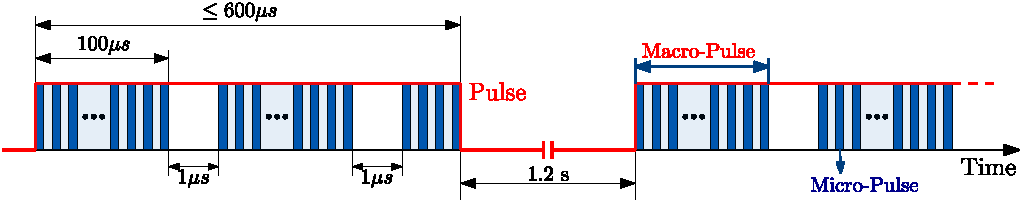
\includegraphics[width=1.0\columnwidth]{Figure_Linac4PulseStructure/Linac4_PulseStruct.pdf}
    \caption{LINAC4 Pulse Structure }
    \label{fig:Linac4PulseStruct}
\end{figure}


\section{Accelerator Physics Principles}
\label{sec:AccPhysPrinc}

The topic of Accelerator physics is very broad, in this section only an overview of the topics of interest for this document will be introduced. These topics include a quick overview of the basic concepts of beam dynamics, transverse plane, beam size and emittance. For a much more complete introduction to the world of accelerator check \parencite*[][]{ref:BookAccPhysics}.

\subsection{Principles of beam dynamics}
\label{subsec:PrincBeamDyn}

For describing the movement of the particles in an accelerator, the Frenet-Serret coordinate system, shown in figure \ref{fig:CoordinateSystem}, is commonly used. S defines the longitudinal coordinate and it is always tangent to the reference path. X and Y define the transverse plane (orthogonal to the particle trajectory). x(s) and y(s) describe the particle's deviation from the reference path at each point. $\rho(s)$ commonly defines the curvature of the reference orbit at each point. 


\begin{figure}[h]
    \centering
    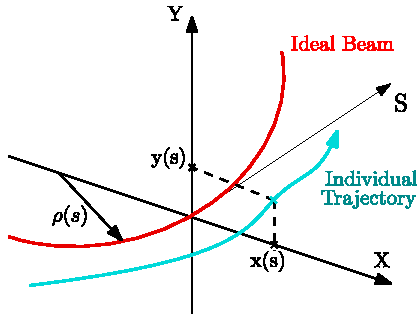
\includegraphics[width=0.5\columnwidth]{Figure_CoordinateSystem/CoordinateSystem.pdf}
    \caption{Frenet-Serret coordinate system.}
    \label{fig:CoordinateSystem}
\end{figure}

The theoretical conception of an accelerator starts by assuming constant energy and a stable beam trajectory. The scope of a particle accelerator design is to guide the beam of particles along the reference path and accelerate them to the desired energy. This is achieved by applying electromagnetic forces to the charged particles. Lorentz's law describes the force acting on a particle of charge "q" traveling in an electromagnetic field:

\begin{equation}
    \vec{F} = q \left( \vec{E} + \vec{v} \times  \vec{B}\right)
    \label{eq:LorentzLaw}
\end{equation}

Where $\vec{E}$ and $\vec{B}$ are the electric and magnetic fields and $\vec{v}$ is the particle velocity. Longitudinal electric fields accelerate the particles, while the transverse bending and focusing are provided by transverse magnetic fields. 

Particles which at the time $t_0$ have a non zero transverse coordinate $\left(x_0 , y_0 \right)$ and momentum $\left(x_{0}^{'} , y_{0}^{'} \right)$ start to perform oscillations in the horizontal and vertical planes,  called Betatron oscillations \parencite*[][]{ref:BookAccPhysics2}. These oscillations depend on the magnetic fields in the ring. The equation of motion on the transverse space can be derived from Lorentz's equation, and after some approximations it reads \parencite*[][]{ref:ApproxEqMotion}:

\begin{equation}
    \begin{aligned}
        x^{''} + \left(\frac{1}{\rho^{2}(s)}+\frac{1}{B\rho}\frac{\partial B_y(s)}{\partial x} \right)  x = 0 \\
        y^{''} - \frac{1}{B \rho}\frac{\partial B_y (s)}{\partial x}  y = 0
    \end{aligned}
    \label{eq:EqMotion}
\end{equation}


The product $B \rho$ is the magnetic rigidity and is equal to the ratio of the momentum to charge $p/q$. The only difference between the vertical and horizontal coordinates is the term $1/\rho^2(s)$ which is related to the centripetal force in the radial direction. These types of differential equations are often referred to as Hills equation \parencite*[][]{ref:HillEquation}, and describe a pseudo harmonic oscillator in which the spring constant depends on the position (s). For each element on the beamline, one can calculate the solution of the equation of motion. The solution of the equation can be expressed in a matrix formulation \parencite*[][]{ref:MatrixForm}:

\begin{equation}
    \begin{bmatrix}
        u(s) \\ u^{'}(s) 
   \end{bmatrix}
   = 
   \begin{bmatrix}
        C(s) & S(s) \\ C^{'}(s)  & S^{'}(s)
   \end{bmatrix}
   \begin{bmatrix}
        u_0 \\ u^{'}_0
   \end{bmatrix}
   =
   M(s) 
   \begin{bmatrix}
        u_0 \\ u^{'}_0
   \end{bmatrix}
\end{equation}

Where $M(s)$ is called the transformation matrix, which can be calculated individually for each type of beamline element. This matrix formalism is very useful as one can follow a particle trajectory along a complicated beam line by repeated matrix multiplication from element to element \parencite*[][]{ref:MatrixTransport}. Three commonly used transport matrices would be the following: 

\begin{itemize}
    \item Drift (no magnetic elements) of length L:
    
    \begin{equation}
        M_D
        =
        \begin{pmatrix}
             1 & L \\ 0 & 1
        \end{pmatrix}
    \end{equation}

    \item Focusing Quadrupole: 
    
    \begin{equation}
        M_{QF} =
        \begin{bmatrix}
             cos\left(\sqrt{k}L_Q\right) & \frac{1}{\sqrt{k}}sin\left(\sqrt{k}L_Q\right) \\
             -\sqrt{k}sin\left(\sqrt{k}L_Q\right) & cos\left(\sqrt{k}L_Q\right)
        \end{bmatrix}
    \end{equation}

    \item Defocusing Quadrupole:
    
    \begin{equation}
        M_{QD} =
        \begin{bmatrix}
             cosh\left(\sqrt{\left|k\right|}L_Q\right) & \frac{1}{\sqrt{\left|k\right|}}sinh\left(\sqrt{\left|k\right|}L_Q\right) \\
             -\sqrt{\left|k\right|}sinh\left(\sqrt{k}L_Q\right) & cosh\left(\sqrt{\left|k\right|}L_Q\right)
        \end{bmatrix}
    \end{equation}

\end{itemize}

In these equations, $L_Q$ refers to the length of the magnets and k is the effective focusing strength of the quadrupoles. 


\subsection{Particle beams and beam profile}
\label{subsec:TransBeamProf}

A beam or a bunch of particles is a collection of a very large number of particles whose center of gravity moves in a well-defined direction. If we consider the transverse plane X-Y (orthogonal to the beam direction of motion), one can obtain the particle distribution by noting the position of each particle that crosses this plane. If there is no coupling between the motion of the particles in the x and y directions, the distribution of the particles will be somehow elliptical, with the axis of the ellipse parallel to the x and y axes. See Figure \ref{fig:TransversePlane} for an example of transverse space particle distribution. 

\begin{figure}[h]
    \centering
    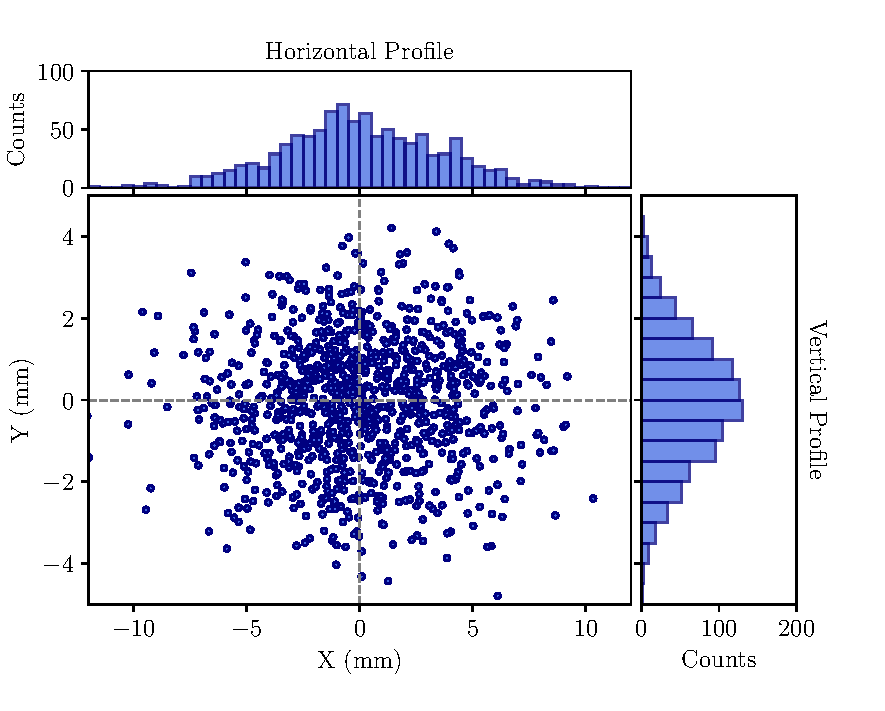
\includegraphics[width=0.9\columnwidth]{Figure_ParticlePositionExample/ParticlePosition.pdf}
    \caption{Example of Particle distribution in the X-Y space, with their corresponding projections.}
    \label{fig:TransversePlane}
\end{figure}

A histogram expressing the number of particles in a beam as a function of the transverse position is known as a beam profile. A Horizontal beam profile gives information about the number of particles at different x positions. A Vertical beam profile gives information about the number of particles at different y positions. 

A typical way of expressing the number of particles at a certain point in space is using a gaussian function:

\begin{equation}
    N(x,y) = \frac{N_{Tot}}{2\pi\sigma_x \sigma_y}\cdot exp\left(-\frac{1}{2}\left(\left(\frac{x-x_0}{\sigma_x}\right)^2 -\left(\frac{y-y_0}{\sigma_y}\right)^2\right)\right)
    \label{eq:GaussianDist}
\end{equation}

Here $x_0 , y_0$ are the coordinates of the center of the beam. $\sigma_x , \sigma_y$ are the standard deviation of the normally distributed beam of particles. $N_{Tot}$ refers to the total number of particles in the beam pulse. However, this expression is no more than an approximation, and one should be careful to understand its limitations. Usually, at the particle source, the beam of particles is far from Gaussian, but after some acceleration, this becomes a good approximation \parencite*[][]{ref:BookAccPhysics}.

\subsection{Transverse phase space}
\label{subsec:TransPhSp}

Each one of the particles in the beam will not only have a different position, but also a different direction of movement. The velocity vector of each particle can be decomposed into two components, one parallel to the beam direction (s) and one orthogonal to it (transverse velocity). The transverse velocity can then be discomposed into its components along the x-axis and y-axis. The phase space has information on both the position and the transverse velocity of each of the particles in the beam. Because the velocity and the momentum of the particles are related, one can express the information of the phase space in terms of the transverse momenta of the particles $\left(p_x , p_y \right)$. 

For convenience, the phase space is described by the transverse momentum $(p_x , p_y)$ normalized by the longitudinal momentum $(p_s)$. This quantities are expressed by: $x^{'} = p_x / p_s$ and $y^{'} = p_y / p_s$. For reprsenting the phase space, two charts are needed, one for the vertical plane and one for the horizontal plane. Figure \ref{fig:PhaseSpace} shows an example of particle distribution in the phase space. 

\begin{figure}[h]
    \centering
    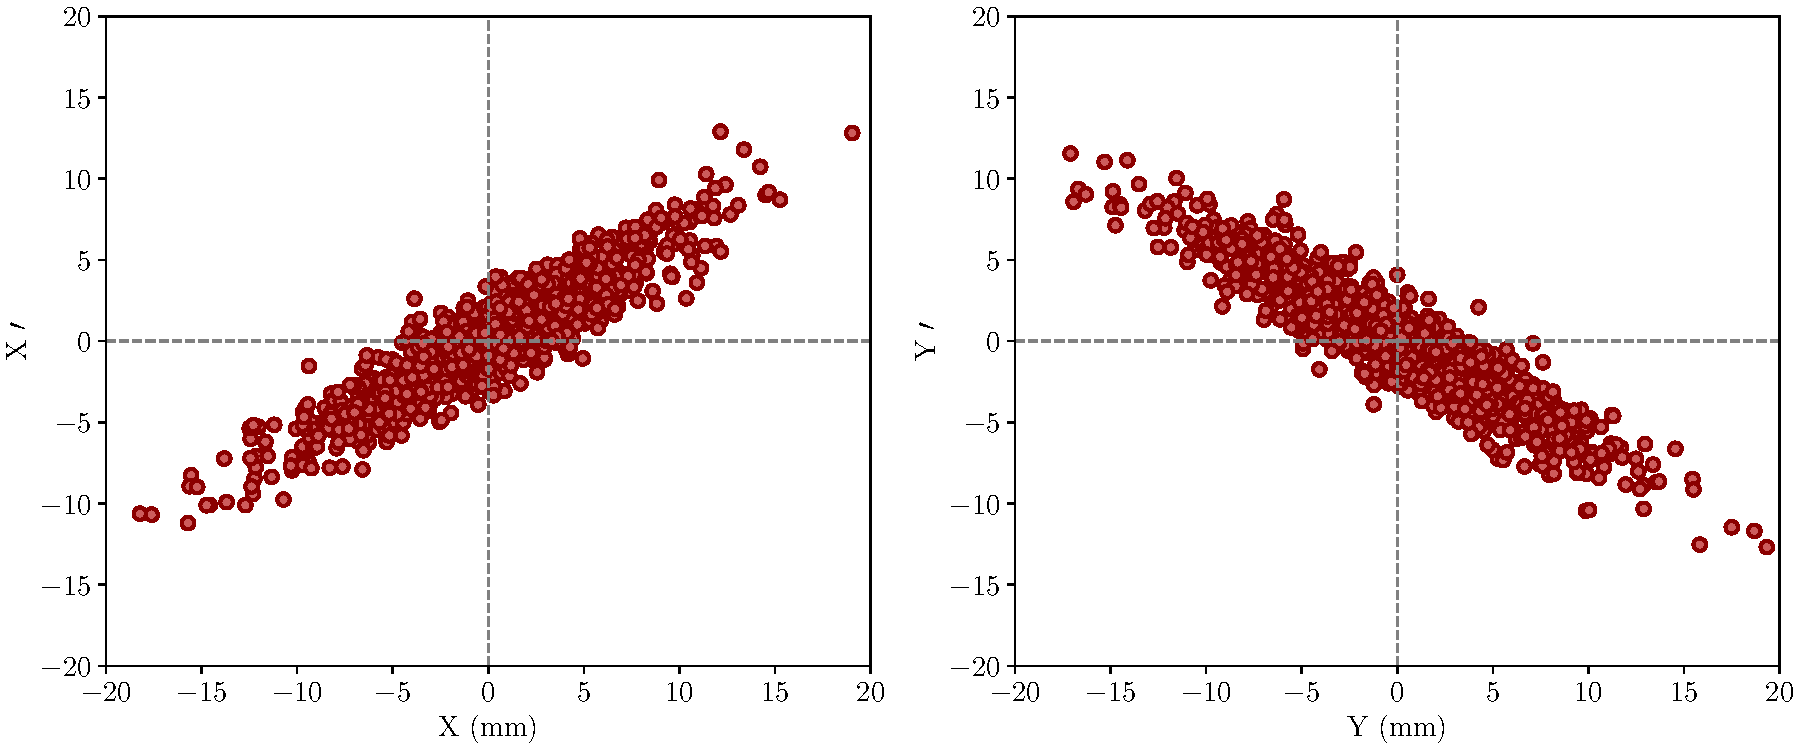
\includegraphics[width=1.0\columnwidth]{Figure_PhaseSpaceDist/PhaseSpaceDist.pdf}
    \caption{Particle distribution in the transverse phase space. }
    \label{fig:PhaseSpace}
\end{figure}

The particle distributions in the phase space are again ellipses, but in this case, they are tilted with respect to the axes. The phase space contains the whole description of the states of all the particles for a particular plane. This information is needed if one wants to calculate the subsequent motion of the particles in the electromagnetic fields of the accelerator. 

\subsection{Transverse beam emittance}
\label{subsec:TransBeamEm}

A formal description of the phase space can be developed by exploiting the elliptical shape of the phase space. The equation of the phase-space ellipse can be described as follows: 

\begin{equation}
    \epsilon = \gamma x^2 + 2\alpha x x^{'} + \beta x^{'2}
    \label{eq:ellipse}
\end{equation}

The parameters $\alpha, \beta, \gamma$ are referred to as the Courant-Synder parameters \parencite*[][]{ref:BookAccPhysics}. The area of the ellipse is simply $A = \pi \epsilon$. In the accelerator and beam physics language, the area in the phase space ($\epsilon$) containing the particles is called the emittance, statistical emittance, or more precisely it is called the rms-emittance. In the case of Gaussian beams, the concept of rms-emittance can be directly interpreted as the area containing a fraction (f) of ions. For example, it can be proven \parencite*[][]{ref:BookAccPhysics2},  that the curve of area $\epsilon$ should contain a $39\%$ of particles. Table \ref{tab:ParticleProportion} resumes the fraction of particles in a gaussian beam associated with various emittances. 


\begin{table}[h]
    \centering
    \begin{tabular}{cc}
    \hline
    Emittance $\epsilon(f)$ & Particle Fraction ($\%$) \\ \hline
    $\epsilon_{rms}$       & 15                     \\
    $\pi \cdot \epsilon_{rms}$     & 39                     \\
    $2\pi \cdot \epsilon_{rms}$  & 63                     \\
    $4\pi \cdot \epsilon_{rms}$  & 86                     \\
    $8\pi \cdot \epsilon_{rms}$   & 98                     \\ \hline
    \end{tabular}
    \caption{Fraction (f) of particles in a Gaussian beam associated with different definitions of emittance.}
    \label{tab:ParticleProportion}
\end{table}

\begin{figure}[h]
    \centering
    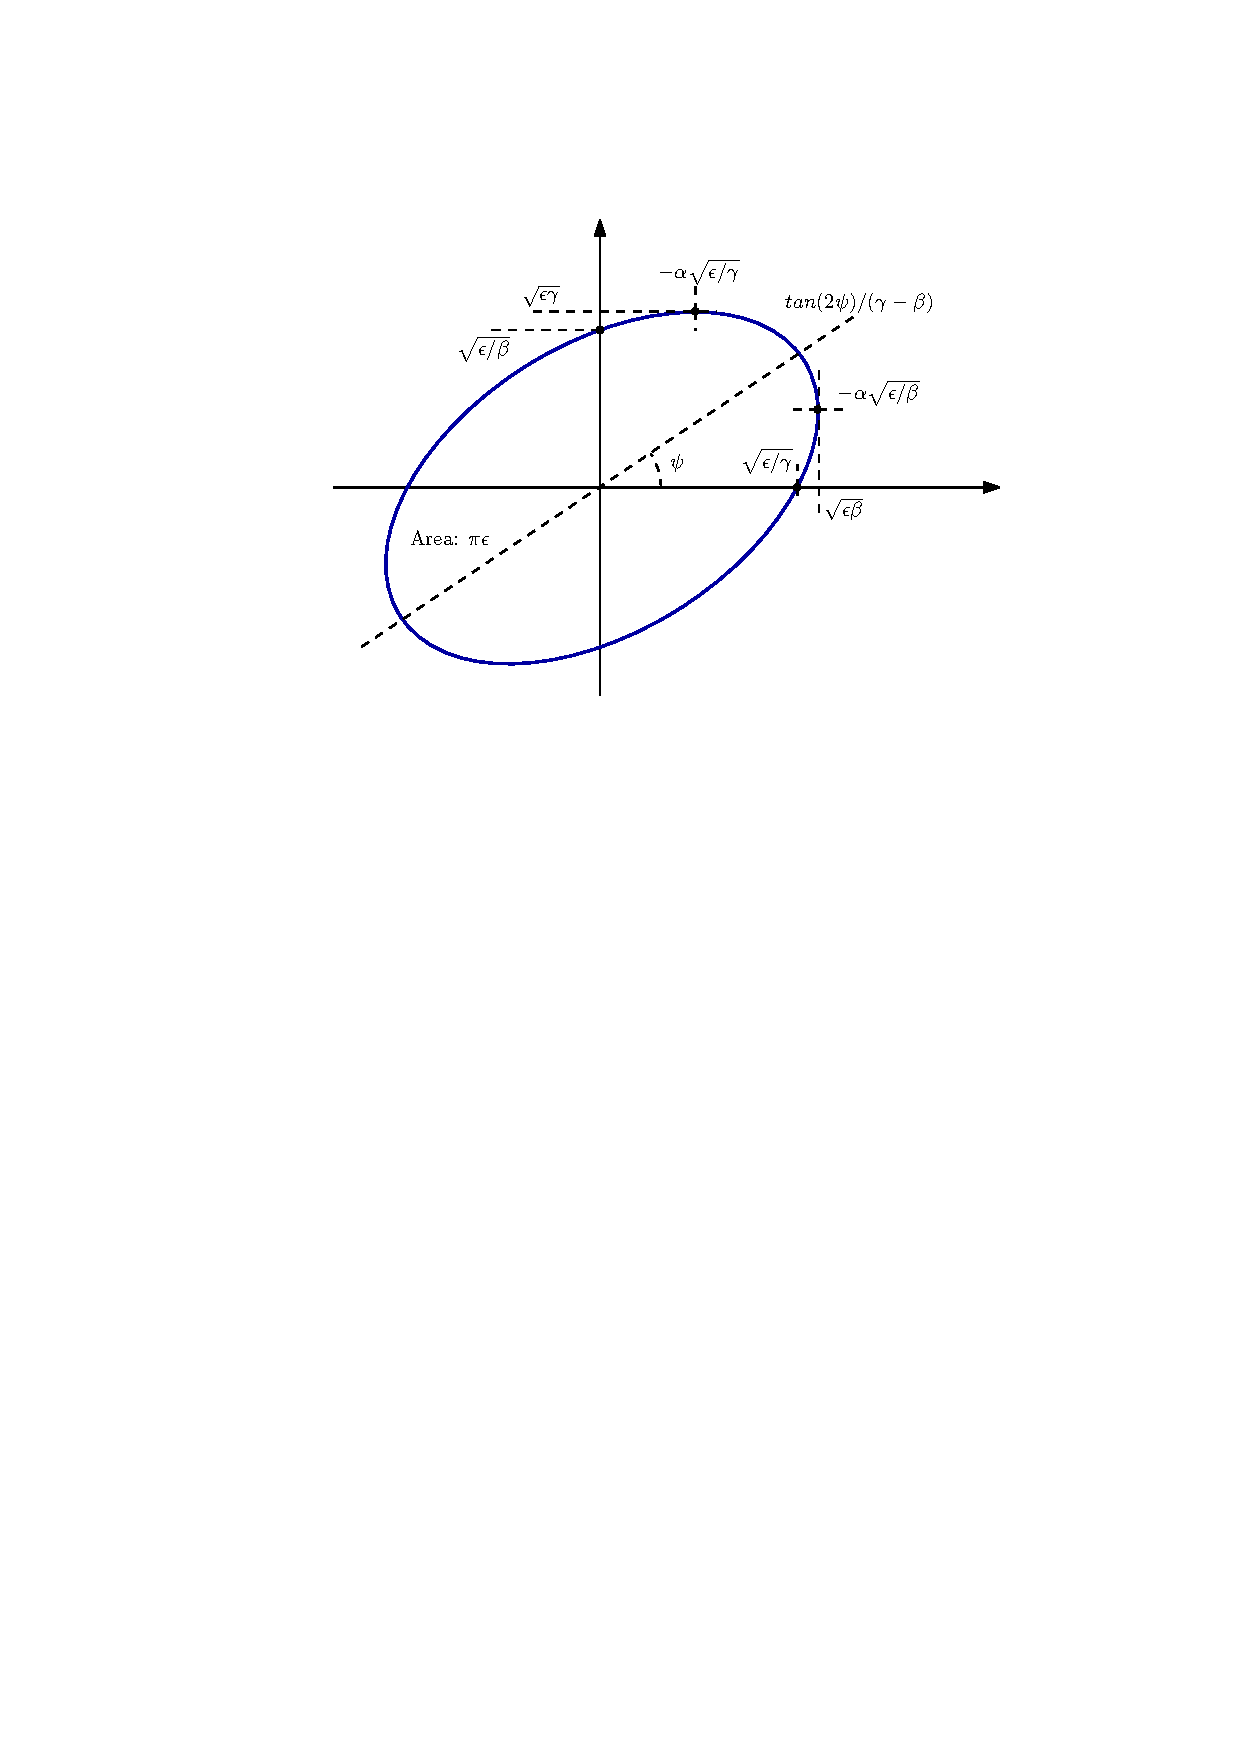
\includegraphics[width=0.7\columnwidth]{Figure_GeometricEmittance/GeometricEmittancve.pdf}
    \caption{Phase Space, geometrical ellipse. }
    \label{fig:CouranSnyder}
\end{figure}

    
Figure \ref{fig:CouranSnyder} shows a geometrical description of the Courant-Snyder parameters. These parameters $\left(\alpha , \beta , \gamma \right)$ are not independent, the third parameter is typically defined in therms of the other two: 

\begin{equation}
    \gamma = \frac{1 + \alpha^{2}}{\beta}
\end{equation}

Some other quantites, also very important for the understanding of the mathematical formulation of the transverse emittance are the following: 

\begin{equation}
    x_{rms}^2 = \left<x^2\right> =\frac{1}{N}\sum_{i=1}^N x_i^2
\end{equation}
\begin{equation}
    x_{rms}^{'2} = \left<x^{'2}\right> = \frac{1}{N}\sum_{i=1}^N x_i^{'2}
\end{equation}
\begin{equation}
    x x^{'}_{rms} =  \left< x x^{'}\right> = \frac{1}{N}\sum_{i = 1}^{N} x_{i} x^{'}_{i}
\end{equation}

With $x_{i} = X_{i} - \left< X \right>$ and $x^{'}_{i} = X_{i} - \left< X^{'}\right>$. $X_{i}$ and $X_{i}^{'}$ being the horizontal position and momentum of the individual particles conforming the beam. For convenience this parameters can be expressed in a matrixs form as follows: 

\begin{equation}
    \Sigma = 
    \begin{pmatrix}
        \left< x^{2} \right> & \left< x x^{'} \right> \\
        \left< x x^{'} \right> & \left< x^{' 2} \right>
    \end{pmatrix}
    = \epsilon 
    \begin{pmatrix}
        \beta & - \alpha \\ -\alpha  & \gamma
    \end{pmatrix}
\end{equation}

The rms-emittance ($\epsilon$) can also be obtained from this parameters as follows: 

\begin{equation}
    \epsilon = \pi \sqrt{\left<x^{2}\right>\left< x^{'2}\right> - '\left<x x^{'}\right>^{2}}
\end{equation}

\subsection{Phase Space Evolution}
\label{subsec:PhaseSpaceEvol}

In a transfer line or a storage ring (i.e. no acceleration), and assuming no energy losses due to radiation, Liouville's theorem establishes that emittance ( considering both transverse and longitudinal coordinates) is conserved \parencite*[][]{ref:EmittanceConserv}. However, the shape of the ellipse changes along the beam line. Figure \ref{fig:PhasSpaceEvol} illustrates a typical example of phase space evolution. 

\begin{figure}[h]
    \centering
    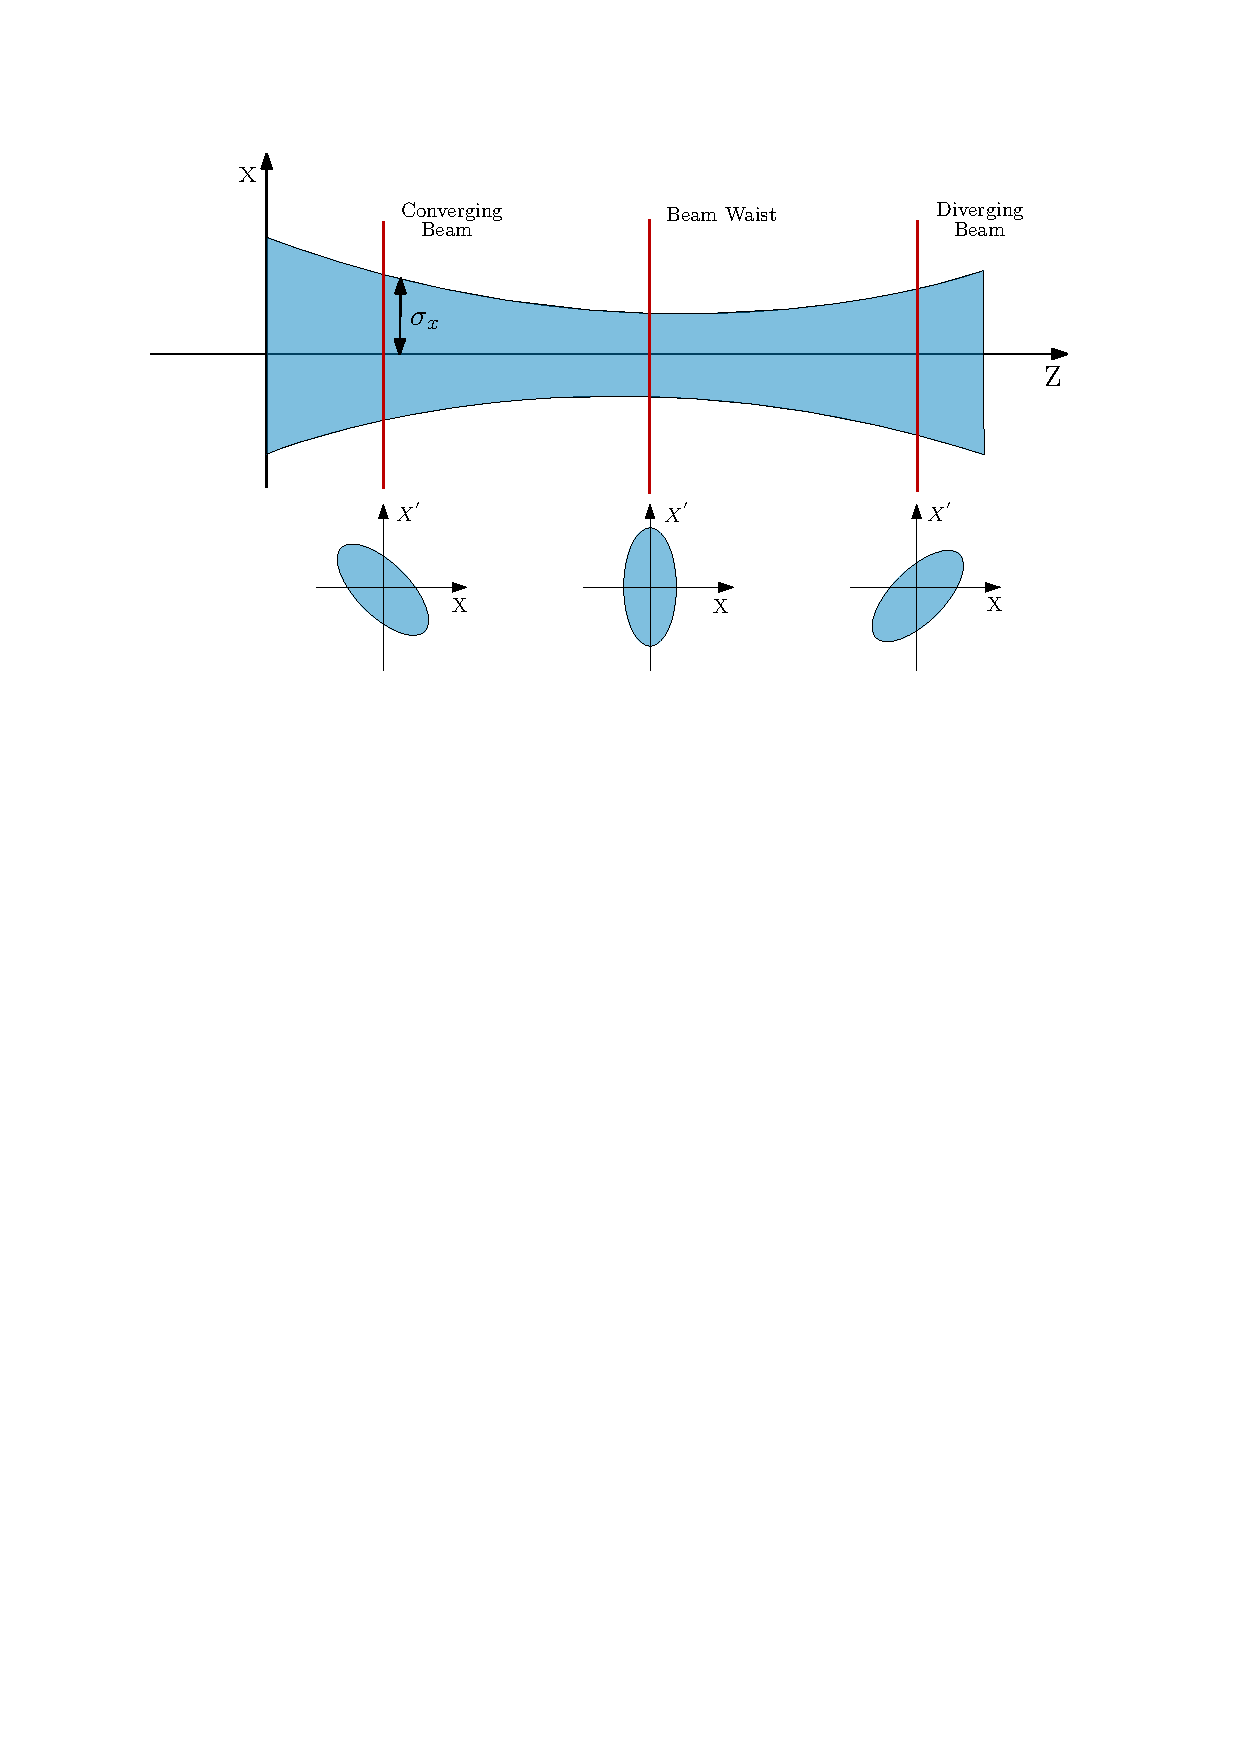
\includegraphics[width=0.9\columnwidth]{Figure_BeamEvolution/BeamEvolution.pdf}
    \caption{Example of phase space evolution. }
    \label{fig:PhasSpaceEvol}
\end{figure}

In the previous sections (Sec. \ref{subsec:PrincBeamDyn}) we saw how, in linear systems, points on the phase-space could be mapped from one location to the other through matrix multiplications. Similarly, assuming the following single-particle transport matrix:

\begin{equation}
    \begin{bmatrix}
         x_1 \\ x_1^{'} 
    \end{bmatrix}
    = 
    \begin{bmatrix}
       c & s \\ c^{'} & s^{'}
     \end{bmatrix}
     \begin{bmatrix}
        x_0 \\ x_0^{'}
     \end{bmatrix}
\end{equation}

After some algebraic calculations, one can obtain the following transport matrix for the Twiss parameters \parencite*[][]{ref:MatrixToTwiss}:

\begin{equation}
    \begin{bmatrix}
       \beta_1 \\ \alpha_1 \\ \gamma_1
    \end{bmatrix}
    =
\begin{bmatrix}
   c^2 & - c s & s^2 \\ -c c^{'} & cs^{'} + c^{'}s & -s s^{'} \\ c^{'2} & -2c^{'}s^{'} & s^{'2}
\end{bmatrix}
=
\begin{bmatrix}
   \beta_0 \\ \alpha_0 \\ \gamma_0
\end{bmatrix}
\label{eq:MatrixEq}
\end{equation}


